\clearpage
\section{Trh práce (definice, nabídka práce, poptávka po práci, rovnováha na trhu práce,
nedokonalosti na trhu práce, nezaměstnanost).}

\subsection{Definice}
\begin{itemize}
    \item Rozhodování mezi volným časem a prací, určujeme si tím hodnotu volného času.
    \item Člověk nabízí svůj čas a za odměnu dostane mzdu. Ta je zároveň i důchodem.
\end{itemize}

\subsection{Nabídka práce}
\begin{itemize}
    \item Substituční efekt - při růstu mzdy chce člověk pracovat více
    \item Důchodový efekt - při růstu mzdy preferuje člověk svůj volný čas
    \item Projevují se oba, při různých výších mzdy, vzniká zpětně zakřivený průběh.
    \item Odvozena od poptávky po volném čase (kolik hodin člověk nechce jako volný čas, 
    tolik může pracovat).
\end{itemize}
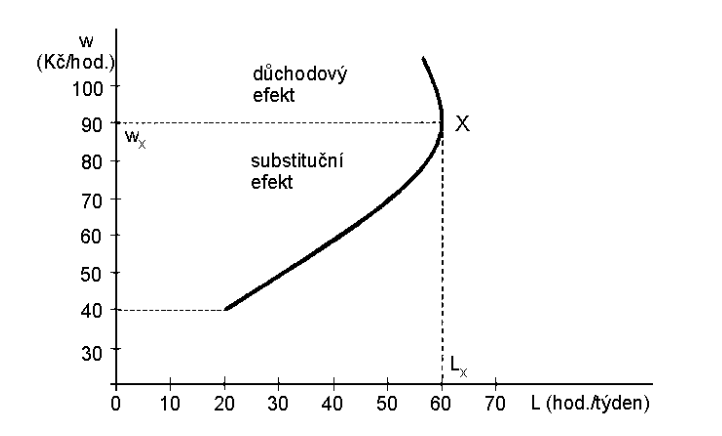
\includegraphics[width=16cm]{images/17_subs_duch_ef.png}

\subsection{Poptávka po práci}
\begin{itemize}
    \item Kolik práce firma najímá při různých cenách práce
    \item $MRP_L=MFC_L=w$, kde $MRP_L$ je příjem z mezního produktu práce, $MFC_L$ jsou
    mezní náklady na práci, $w$ je mzdová sazba 
\end{itemize}
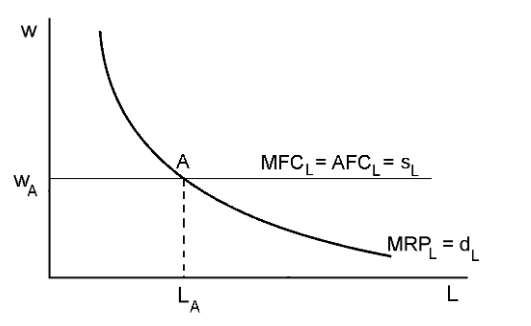
\includegraphics[width=16cm]{images/17_poptavka_po_praci.png}

\subsection{Rovnováha na trhu práce}
\begin{itemize}
    \item Průsečík poptávky a nabídky
    \item Mzdová sazba pod rovnovážným bodem vyvolá nedostatek pracovních sil (nezájem o práci).
    Jejich počet je dán úsečkou $CD$
    \item Nad bodem rovnováhy vzniká přebytek pracovních sil, nezaměstnanost, počet nezaměstnaných 
    je dán úsečkou $AB$.
\end{itemize}
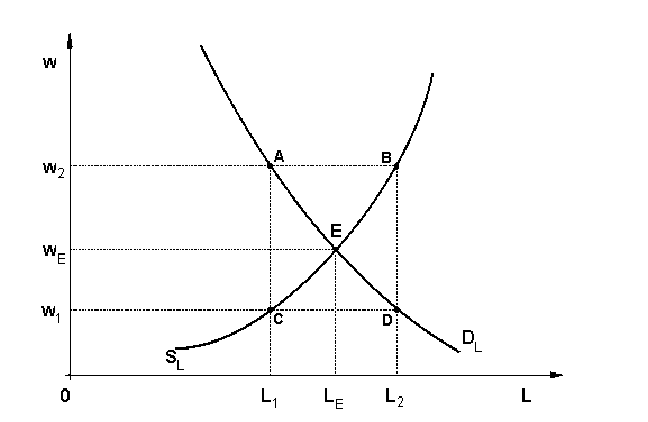
\includegraphics[width=16cm]{images/17_rovnovaha.png}

\subsection{Nedokonalosti na trhu práce}
\subsubsection{Na straně nabídky}
\begin{itemize}
    \item Strukturální různorodost - trhy nejsou konkurenční (lékaři a piloti se vzájemně nezastoupí)
    \item Diskrétnost nabídky - např. platové stupnice a omezení pracovní doby
    \item Mimoekonomické vlivy - aktivita odborů, regulační aktivita vlády
\end{itemize}
\subsubsection{Na straně poptávky}
\begin{itemize}
    \item Právní předpisy
    \item Kolektivní smlouvy
\end{itemize}

\subsection{Nezaměstnanost}
\begin{itemize}
    \item Kdo nemá práci a hledá ji
    \item Jak zjistit nezaměstnanost:
    \begin{enumerate}
        \item Registrovaná nezaměstnanost - nahlásí se na úřad práce,\\
        $$ Nezaměstnanost= \frac{Nezaměstnaní}{Všichni} \cdot 100 \% $$
        \item Pomocí výběrového šetření pracovních sil, nezaměstnaní podle ní jsou osoby starší 15 let, které nebyly zaměstnané, hledaly aktivně práci různými způsoby a byly připraveny k nástupu do práce nejpozději do 14 dnů.
    \end{enumerate}
    \item Metody se liší, protože ne každý registrovaný nezaměstnaný nepracuje (práce \uv{na černo}) 
\end{itemize}